\documentclass[border = 0.2cm, 12pt]{standalone}
\usepackage{amsmath, amssymb, amsfonts}
\usepackage{color}
\usepackage{tikz, pgfplots}
\pgfplotsset{compat=newest}
\usetikzlibrary{shapes,snakes}
\tikzset{>=latex}
\usetikzlibrary{angles,quotes}
\usepackage{tkz-euclide}

\begin{document}

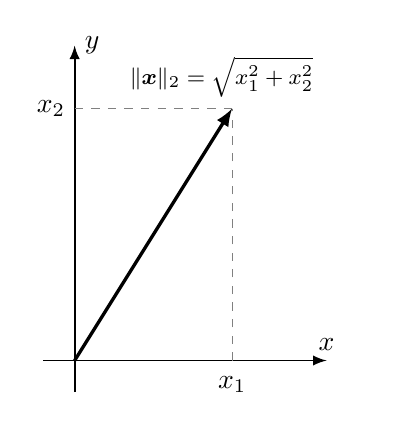
\begin{tikzpicture}[scale=2]

\draw[->,line width=0.7] (-0.2,0)--(1.6,0) node[above]{$x$};
\draw[->,line width=0.7] (0,-0.2)--(0,2) node[right]{$y$};

\draw[arrows=->, line width=1.2] (0,0)--(1,1.6);
\draw[dashed, color=gray, thin] (1,0)--(1,1.6);
\draw[dashed, color=gray, thin] (0,1.6)--(1,1.6);

\node[text width=3cm] at (1.1,1.8) {\footnotesize $\|\boldsymbol{x}\|_2=\sqrt{x_1^2+x_2^2}$};

\node at (1,-0.15) {$x_1$};
\node at (-0.15,1.6) {$x_2$};

\end{tikzpicture}

\end{document}